\section{Gradient methods - Part I}

\begin{definition}[smoothness]
	The function $f : \mathbb{R}^{n}\rightarrow \mathbb{R}$ is $L$-smooth
	if $\nabla f(x)$ satisfies
	\[|\nabla f(x)-\nabla f(y)|\le L|x-y| \quad \forall x,y \in \mathbb{R}^{n}\]
\end{definition}

This result (with Taylors'Theorem) in:

\[f(y)\le f(x)+\nabla f(x)\T (y-x) +\frac{L}{2}|x-y|^2 \quad \forall x,y \in \mathbb{R}^{n}\]

\begin{definition}[strong convexity]
	The function $f : \mathbb{R}^{n}\rightarrow \mathbb{R}$ is $\mu$-strongly convex
	if it satisfies

	\[f(y)\ge f(x)+\nabla f(x)\T (y-x) +\frac{\mu}{2}|x-y|^2 \quad \forall x,y \in \mathbb{R}^{}\]
\end{definition}

\subsection{Gradient Descent}

Given $x_0$ and stepsize $T$ > 0

$\quad x_{k+1}=x_k - T\nabla f(x_k)\quad$for$\ k = (k_0,\dots,k_N)$

% \usepackage{listings}
% \begin{lstlisting}[language=Python]
% def gradient_descent(x_0, T):
%   for k in range(N):
%     x_next = x - T * df(x)
% \end{lstlisting}

\begin{verbatim}
def gradient_descent(x_0, T):
  for k in range(N):
    x_next = x - T * df(x)
\end{verbatim}

% The variable \texttt{x = 1} is initialized
%
% The code \verb|x = 1| sets the value.

HERLEITUNG

Assume
$f(x)=c_0+b\T x+\frac{1}{2}x\T Hx$,
$H\succ0$
$\Rightarrow$
$Hx^\star =-b$

$x_{k+1}-x^\star=x_k-x^\star-T(b+Hx_k)$
$=(I-TH)(x_k-x^\star)$

\[\begin{aligned}
		x_{k+1}-x^\star & =x_k-x^\star-T(b+Hx_k)
		\\
		                & =(I-TH)(x_k-x^\star)
	\end{aligned}\]

Convergence given by eigenvalus of $I-TH$,
use $H=U\Lambda U\T$

$x_{N}-x^\star=$
$U(I-T\Lambda)^N U\T(x_k-x^\star)$
$\rightarrow$
Convergence rate is dictated by $1-T\lambda_i$

\textbf{Optimal Step Size}

$\mu \le h \le L$

\[T^\star = \frac{2}{L+\mu}  \]

GRAFIK

\textbf{Convergence rate}
$$\rho (T^\star) = |1-\frac{2L}{L+\mu}|= \frac{L-\mu}{L+\mu}$$

therefore with stepsize $T^\star$

$|x_N - x^\star| \le \epsilon $
if $N \ge \frac{\kappa+1}{2}\operatorname{ln}(\frac{|x_0 - x^\star|}{\epsilon})$

\subsection{Momentum-based methods}
\begin{equation}
	\begin{aligned}
		q_{k+1} & = q_k + Tp_{k+1}                          \\
		p_{k+1} & = (1-2dT)p_k-T\nabla f(q_k + \beta p_k)/L
	\end{aligned}
\end{equation}

SPRING DAMPER ANALOGY

Nesterovs accelerated gradient methods

- for $T = 1, d=\frac{1}{\sqrt{k}+1}, \beta =\frac{\sqrt{k}-1}{\sqrt{k}+1}$

Heavy Ball (tuned quadratics)

- for $T = \frac{2\sqrt{k}}{\sqrt{k}+1}, d=\frac{1}{\sqrt{k}+1},\beta =0$


\textbf{What is the convergence rate?}

EXAMPLE DIAGONALIZATION

EIGENVALUE analysis

ROOT Locus

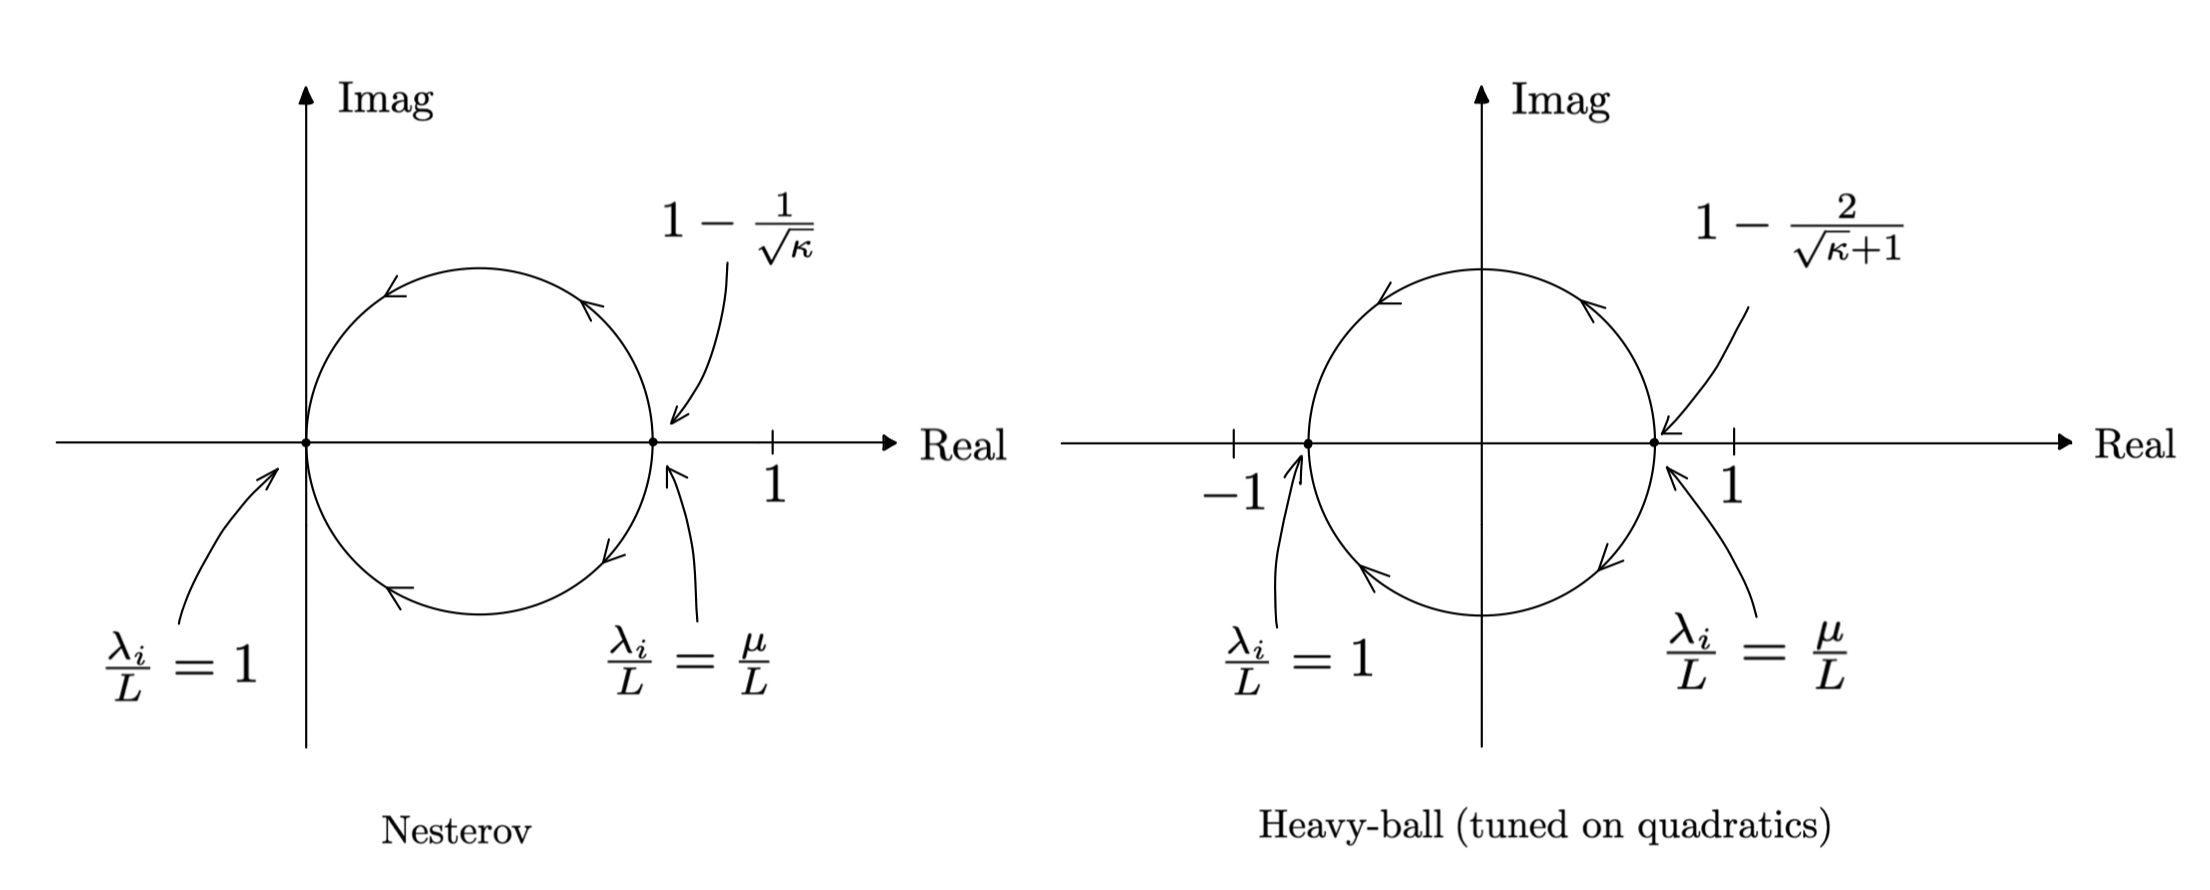
\includegraphics[width=\columnwidth]{images/root-locus-momentum.png}
- Nesterov on circle $c=(r/0), r=\lambda_i/L = \mu /L$

- Heavy ball circle $c=((\lambda -L)/2 ,0), r= \lambda +L$

\centering{
	$C_\text{Nesterov}(1-\frac{1}{\sqrt{\kappa}})^N$
	$\approx\frac{|q_N-q^\star|}{|q_0-q^\star|}\approx$
	$C_\text{HeavyBall}(1-\frac{2}{\sqrt{\kappa+1}})^N$
}

Requires
$N\ge2\sqrt{\kappa}\operatorname{ln}(\frac{|q_{0}-q^\star|}{\epsilon})$
to achieve
$|x_{N}-x^\star|\le\epsilon$

\begin{theorem}
	For any first-order method
	$\exists f: \mathbb{R}^{\infty}\rightarrow\mathbb{R}$,
	$\mu$-scv, $L$-sm,
	s.t.
	$|x_k - x^\star|\ge$
	$(1-\frac{2}{\sqrt{\kappa}+1})^k|x_0 - x^\star| \forall k\ge 0$

\end{theorem}

%TODO: proof with H Function

